\documentclass[professionalfonts,svgnames]{beamer}
\usepackage[czech]{babel}
\usepackage[utf8]{inputenc}
\usepackage{fontenc}
\usepackage{graphicx}
\usepackage{verbatim}

% Definice použité barvy
\definecolor{umk}{RGB}{164,0,0}

% Obarveni titulní stránky
\setbeamercolor{title}{fg=umk}
\setbeamercolor{frametitle}{fg=umk}
\setbeamercolor{item}{fg=umk}
\setbeamercolor{alerted text}{fg=umk}

% Nastaveni daného fontu
\usebeamerfont{lmodern}
\setbeamertemplate{navigation symbols}{}
\setbeamerfont{frametitle}{family=\bf}
\setbeamerfont{title}{family=\bf}

% Nastaveni titulku prezentace
\title{\texorpdfstring{Co by měl každý programátor vědět o počítačové paměti}{Co by mel kazdy programator vedet o pocitacove pameti}}
\author{\texorpdfstring{Petr Holášek\newline\small \url{holasekp@gmail.com}}{Petr Holasek}}
\titlegraphic{\includegraphics[width=2cm]{logo-white}}
\institute{\texorpdfstring{Univerzita Mikuláše Koperníka}{Univerzita Mikulase Kopernika}}
\date{23. února 2013}

% Definice odsazení titulku stránky
\setbeamertemplate{frametitle}{\vspace{8mm}\parbox{\textwidth}{\par\usebeamerfont{frametitle}\insertframetitle}}

% Upravení patičky stránky a doplnění pořadí
\setbeamertemplate{footline}{\parbox[c]{0.97\textwidth}{\hfill\tiny\color{gray}(Strana \insertframenumber/\inserttotalframenumber)}\vspace{3mm}}

\begin{document}
%%%%%%%%%%%%%%%%%%%%%%%%%%%%%%%%%%%%%%%%%%%%%%%%%
%%	Frame 1 - Titulek
%%%%%%%%%%%%%%%%%%%%%%%%%%%%%%%%%%%%%%%%%%%%%%%%%
\begin{frame}
\titlepage
\end{frame}
%%%%%%%%%%%%%%%%%%%%%%%%%%%%%%%%%%%%%%%%%%%%%%%%%
%%	Frame 2 - Forma predmetu
%%%%%%%%%%%%%%%%%%%%%%%%%%%%%%%%%%%%%%%%%%%%%%%%%
\begin{frame}
\frametitle{Popis předmětu IMEM}
Přednášky:
\begin{itemize}
\item Jedna přednáška 23.2.2013; 10:00
\end{itemize}
Zkouška:
\begin{itemize}
\item První a poslední termín zkoušky 24.2.2013
\item Full-text + sada otázek na ABCD
\end{itemize}
Hodnocení:
\begin{itemize}
\item 0-49 b. = F
\item 50-59 b. = E, 60-69 b. = D, 70-79 b. = C, 80-89 b. = B, 90-100 b. = A
\end{itemize}
\end{frame}

%%%%%%%%%%%%%%%%%%%%%%%%%%%%%%%%%%%%%%%%%%%%%%%%%

% Uvod
% Co je to pamet
% Pam. hierarchie - projde se
% Operacni system
% Procesy
% Virtualni pamet
% Tabulka stranek
% Programovani v C - jak funguje malloc, brk, mmap, mlock, zobrazeni mapovani aplikace

\begin{frame}
\frametitle{Obsah přednášky}
\begin{enumerate}
\item Paměťová hierarchie
\item Operační systém
\item Virtuální paměť
\item Práce s pamětí z pohledu programátora
\end{enumerate}
\end{frame}


%%%
\begin{frame}
\frametitle{Co je to paměť?}
\begin{itemize}
\item Prostor k uložení dat
\item Různé velikosti a různé rychlosti, platí nepřímá úměra (viz. Paměťová hierarchie)
\item V dnešních operačních systémech je nutné použít pokročilé techniky správy paměti
\end{itemize}
\end{frame}

%%%
\begin{frame}
\frametitle{Paměťová hierarchie}
\begin{itemize}
\item Uspořádání paměťových úložišť:
	\begin{itemize}
		\item Vzestupně podle kapacity
		\item Sestupně podle rychlosti
	\end{itemize}
\item Data se pohybují oběma směry
\item Stupně:
	\begin{itemize}
	\item Registry procesoru
	\item Cache (L1, L2, L3)
	\item Hlavní paměť (RAM - Random Access Memory)
	\item Sekundární úložiště (disk, páska)
	\end{itemize}
\end{itemize}
\end{frame}

%%%
\begin{frame}
\frametitle{Paměťová hierarchie}
\begin{figure}[h]
	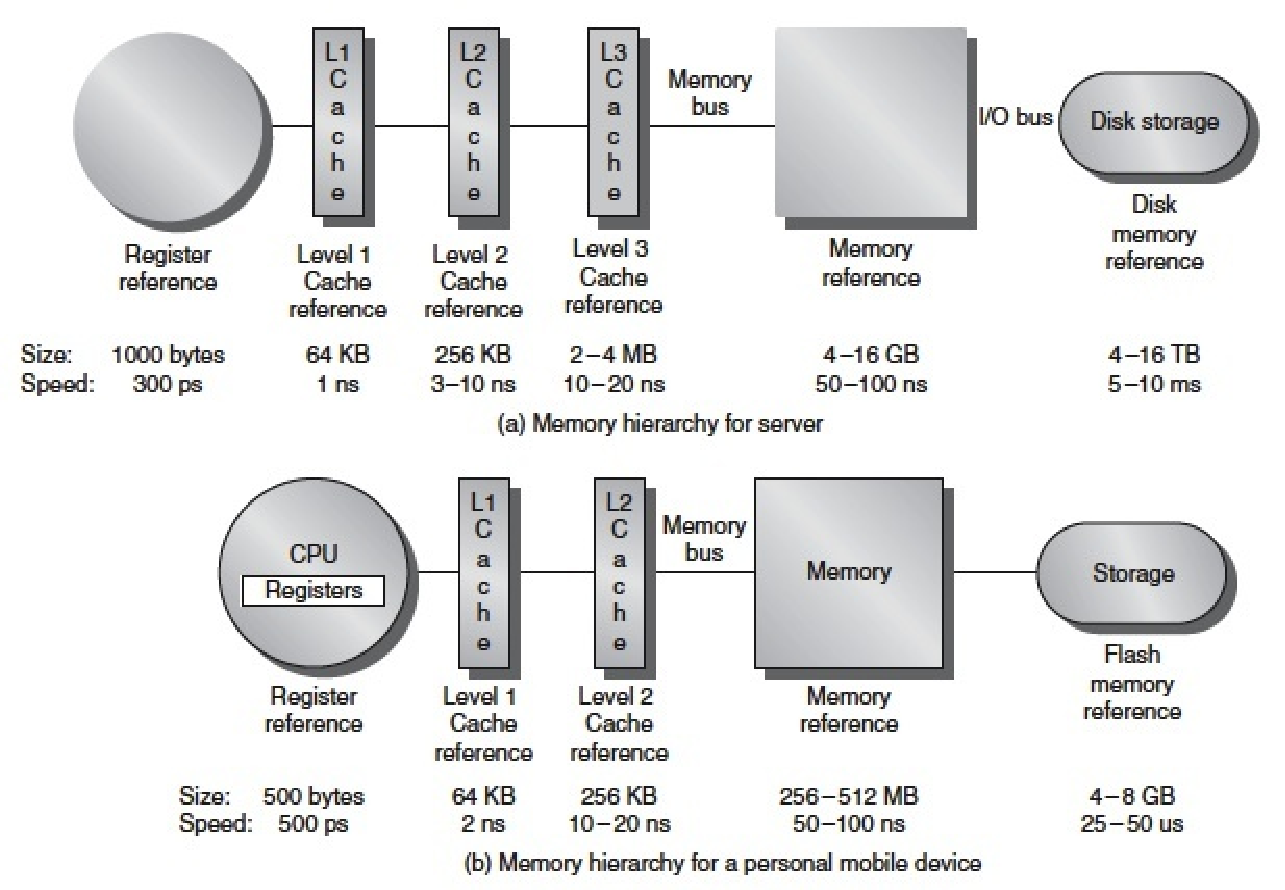
\includegraphics[width=\textwidth,keepaspectratio]{fig/hier}
	\caption{Paměťová hierarchie (zdroj: Hennessy, Patterson)}
	\label{hier}
\end{figure}
\end{frame}

%%%
\begin{frame}
\frametitle{Statická RAM aka SRAM}
\begin{itemize}
\item SRAM je obvykle použita v registrech a cache
\item Výhodnější vlastnosti než DRAM, ale má vyšší spotřebu a její výroba je dražší
\item Stav buňky není potřeba obnovovat, ale je třeba dodávat konstantní proud
\end{itemize}
\begin{figure}[h]
	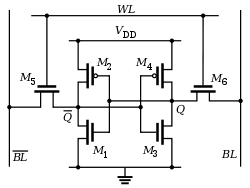
\includegraphics[scale=0.6]{fig/sram}
\end{figure}
\end{frame}

%%%
 \begin{frame}
\frametitle{Dynamická RAM aka DRAM}
\begin{itemize}
\item Použití v hlavní paměti počítače
\item Stav buňky uchován v kapacitoru $C$
\item Nutnost obnovování obsahu buňky každých několik desítek milisekund
\item Buňky jsou obvykle uspořádány v matici, důvodem je velikost paměti ($4GB = 2^{32}$ adres)
\end{itemize}
\begin{figure}[h]
	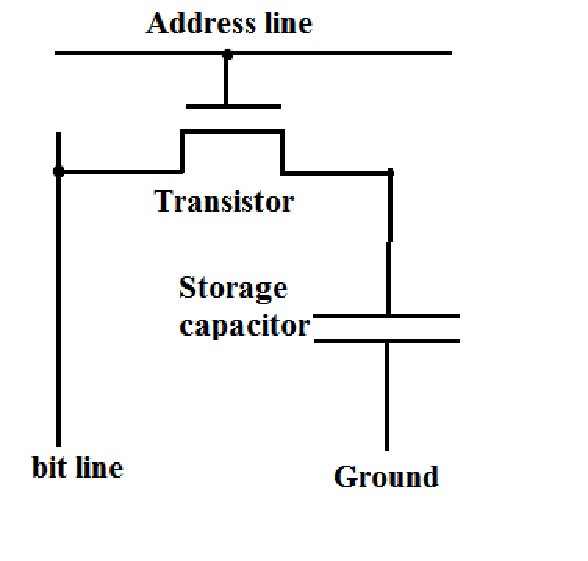
\includegraphics[scale=0.5]{fig/dram}
\end{figure}
\end{frame}

%%%
 \begin{frame}
\frametitle{Registry CPU}
\begin{itemize}
\item Velice malé kusy paměti uvnitř CPU (typicky 32-64 bit podle architektury)
\item eax, ebx, eip, esp, ... (asembleroví labužníci znají, odvážnější linuxisté určitě někdy viděli)
\item Nové sady SIMD instrukcí typu SSE nebo AVX mají svoje vlastní
\end{itemize}
\end{frame}

%%%
 \begin{frame}
\frametitle{Cache}
\begin{itemize}
\item Rychlá a malá paměť mezi CPU a hlavní pamětí pro překlenutí velkého rychlostního rozdílu
\item V nejnovějších procesorech obvykle třístupňová L1-L3
\item Využívá principů \textit{časové} a \textit{místní lokality}
\end{itemize}
\end{frame}

%%%
 \begin{frame}
\frametitle{Uspořádání pamětí cache v dnešních procesorech}
\begin{figure}[h]
	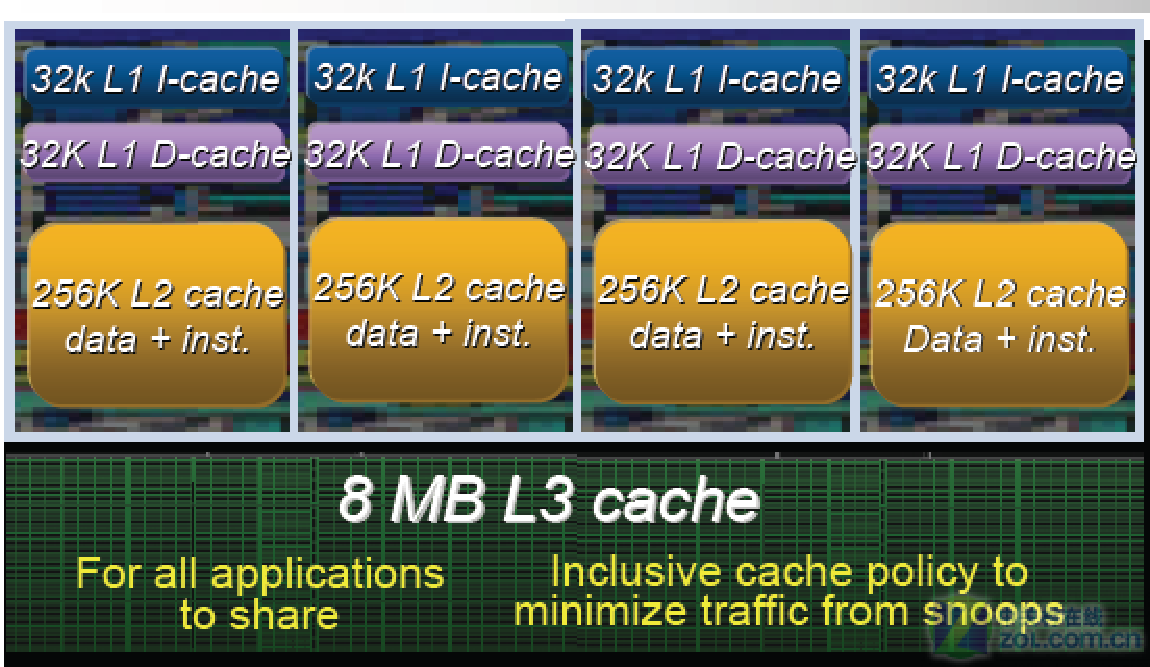
\includegraphics[scale=0.55]{fig/cache}
\end{figure}
\end{frame}

%%%
 \begin{frame}
\frametitle{Adresování dat v cache}
\begin{figure}[h]
	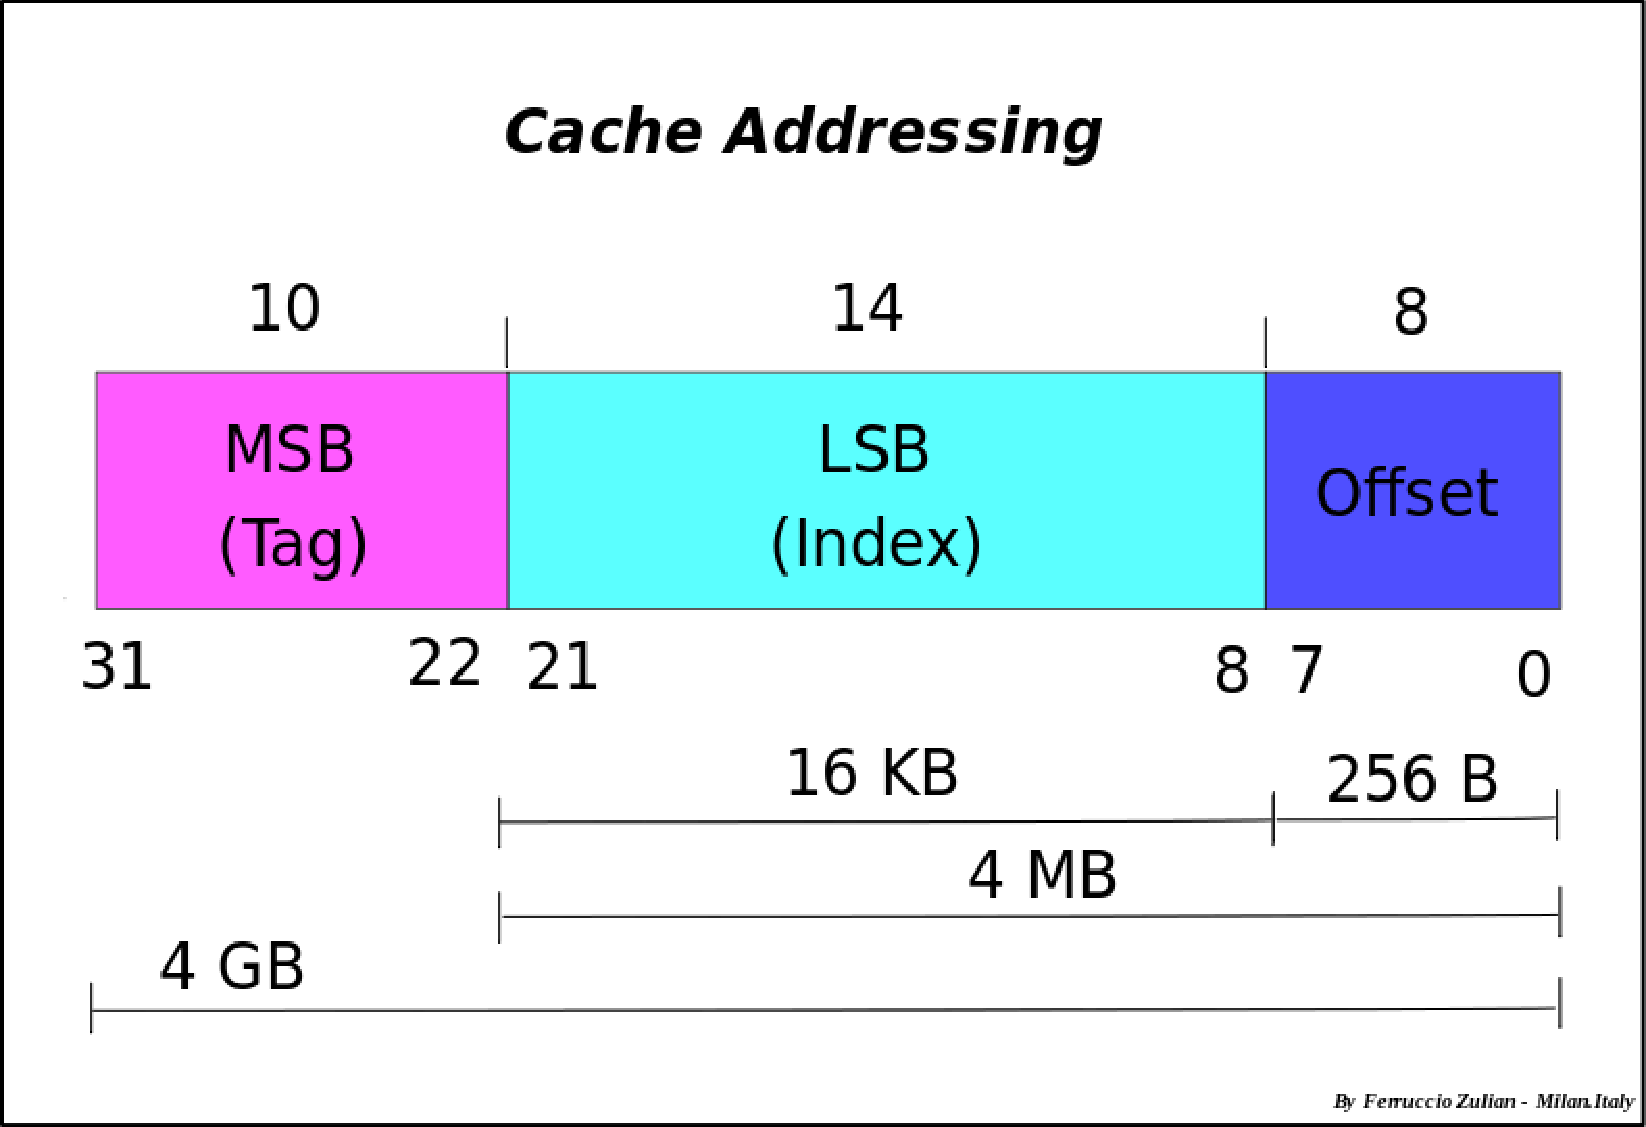
\includegraphics[width=\textwidth,keepaspectratio]{fig/addr}
\end{figure}
\end{frame}

%%%
 \begin{frame}
\frametitle{Asociativita cache}
\begin{itemize}
\item plně asociativní - není třeba index, blok může být umístěn kdekoli v cache, flexibilní co se týče umístění bloků, použitelné pouze u velmi malých cache kvůli
počtu porovnání tagů
\item přímo mapovaná - každý blok může být umístěn pouze na jednom místě v cache, neflexibilní umístění bloků, klasicky modulo
\item kompromisem je \textit{n-cestná cache} - index najde cestu, tag konkrétní blok, kompromisní řešení
\end{itemize}
\end{frame}

%%%
 \begin{frame}
\frametitle{Asociativita cache}
\begin{figure}[h]
	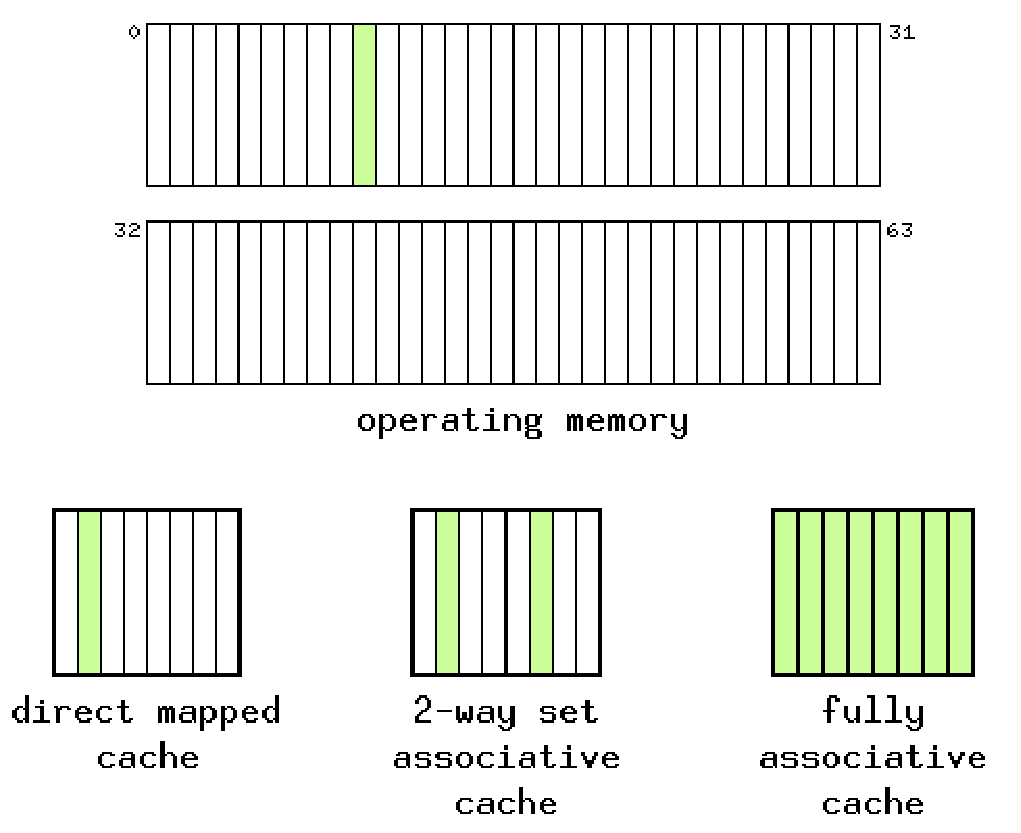
\includegraphics[scale=0.5]{fig/cway}
\end{figure}
\end{frame}

%%%
 \begin{frame}
\frametitle{Metody propagace dat z/do cache}
\begin{description}
\item[write-through] Data jsou zapsány zároveň do bloku cache i do bloku paměti na nižší úrovni.
\item[write-back] Data jsou zapsány pouze do bloku cache. Tento modifikovaný blok je zapsán do hlavní paměti až při jeho výměně.
\end{description}
\end{frame}

%%%
 \begin{frame}
\frametitle{Metriky používané pro paměti cache}
\begin{itemize}
\item \textit{miss rate}
\item \textit{hit rate}
\item \textit{instruction cycles per miss}
\item \textit{instruction cycles per hit}
\item Pro experimenty s Vašimi binárkami:\\ \texttt{valgrind --tool=cachegrind ./muj\_program}
\end{itemize}
\end{frame}

\begin{frame}[fragile]
\frametitle{Cachegrind}
Ukázkový výstup pro quicksort na poli náhodně generovaných 10000 prvku:
\begin{verbatim}
==9471== I   refs:      18,321,256
==9471== I1  misses:    814
==9471== LLi misses:    808
==9471== 
==9471== D   refs: 6,219,587 (3,828,621 rd + 2,390,966 wr)
==9471== D1  misses: 3,723  (2,754 rd   +  969 wr)
==9471== LLd misses: 1,494  (635 rd   +  859 wr)
==9471== 
==9471== LL refs:   4,537  (3,568 rd   +  969 wr)
==9471== LL misses: 2,302  (1,443 rd   +  859 wr)
\end{verbatim}
\end{frame}

%%%
 \begin{frame}
\frametitle{Operační systém}
\begin{itemize}
\item Vrstva mezi HW a uživatelských SW
\item Poskytuje programátorům iluzi, že:
	\begin{itemize}
		\item paměti pro jejich program je nekonečně mnoho
		\item adresy jdou hezky spojitě od $0-N$
		\item jejich proces běží na svém (nebo svých) CPU sám a nepřetržitě
	\end{itemize}
... nicméně jádro OS se zapotí, aby této iluze dosáhlo.
\end{itemize}
\end{frame}

%%%
\begin{frame}
\frametitle{Proces}
\begin{itemize}
\item Jde o zapouzdření běžící aplikace (\texttt{bash}, \texttt{openoffice}, \texttt{gdb}) z pohledu OS
\item Na systému jich může běžet "zároveň" velmi mnoho (desítky tisíc)
\item Každý proces má vlastní lineární paměťový prostor, který může používat:
	\begin{description}
		\item [32-bit] 4GB (proč právě tolik?)
		\item [64-bit] teoreticky 16EB, prakticky v Linuxu 128TB
	\end{description}
\item Procesy jsou postupně přepínány plánovačem jádra tak, aby se každý dostal na určitý čas k procesu
\end{itemize}
\end{frame}

%%%
 \begin{frame}
\frametitle{Stránkování}
\begin{itemize}
\item Na všech moderních OS je nejmenší použitelné množství paměti 1 stránka
\item Typicky 4kB, existují však i větší (viz. hugepages v Linuxu)
\item Z pohledu OS rozlišujeme dva typy stránek:
	\begin{itemize}
		\item Virtuální stránky - viditelné pro běžící procesy a tedy programátory
		\item Fyzické rámce - paměť v RAM
	\end{itemize}
\end{itemize}
\end{frame}

%%%
\begin{frame}
\frametitle{Virtuální paměť}
\begin{itemize}
\item Koncept řešící současný běh více procesů na jednom systému
\item Každý běžící proces má k dispozici 4GB adresového prostoru rozděleného na jednotlivé \textit{stránky}
\item Virtuální paměť řeší přiřazení fyzických rámců ke stránkám virtuálních (ne nutně 1:1 - u sdílených knihoven)
\item Adresa \texttt{0x89f92ad2} u procesu $1$ ukazuje do jiné buňky paměti než stejná adresa u procesu $2$
\end{itemize}
\end{frame}

%%%
%%%
 \begin{frame}
\frametitle{Tabulka stránek}
\begin{itemize}
\item Udržuje mapování virtuálních stránek na fyzické rámce pro \textbf{každý} běžící proces
\item Adresa je rozdělena na několik částí podle počtu stupňů TS a offset
\item Hledání v tabulce je časově náročné, existuje tedy malá cache TLB (Translation lookaside buffer), která obsahuje poslední úspěšné překlady mapování
\item Při přepnutí procesu je TLB vyprázdňována
\end{itemize}
TODO: Obrázek!
\end{frame}

%%%%
\begin{frame}
\frametitle{Tabulka stránek}
\begin{figure}[h]
	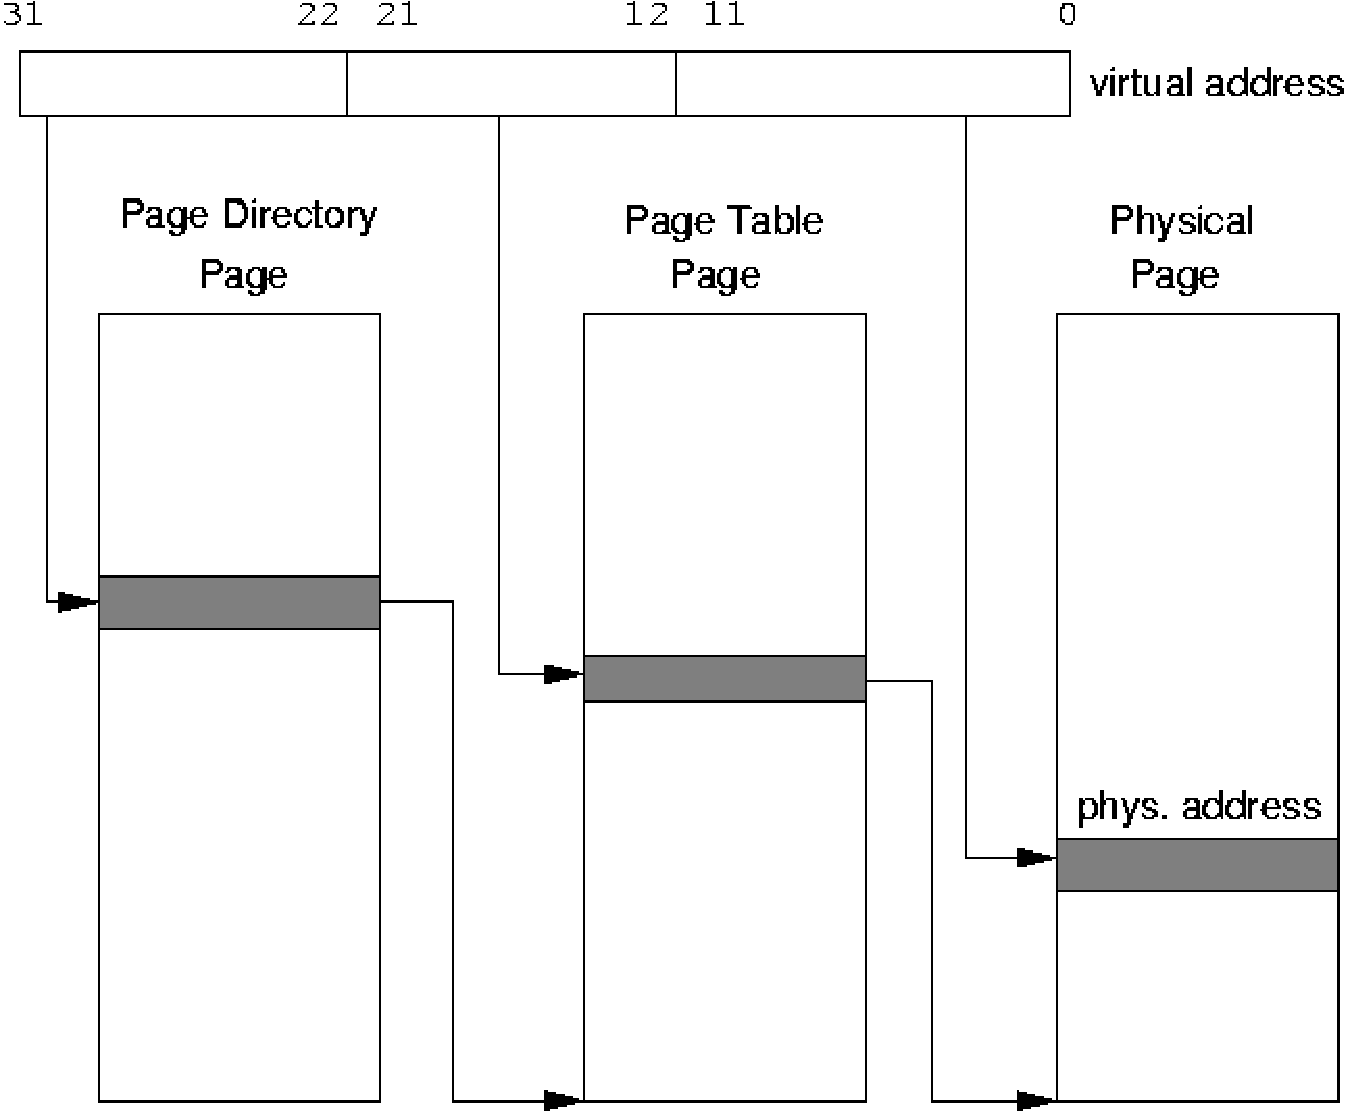
\includegraphics[scale=0.4]{fig/pgtable}
	\caption{Tabulka stránek}
	\label{vm}
\end{figure}
\end{frame}

%%%%
\begin{frame}
\frametitle{Překlad adres}
\begin{figure}[h]
	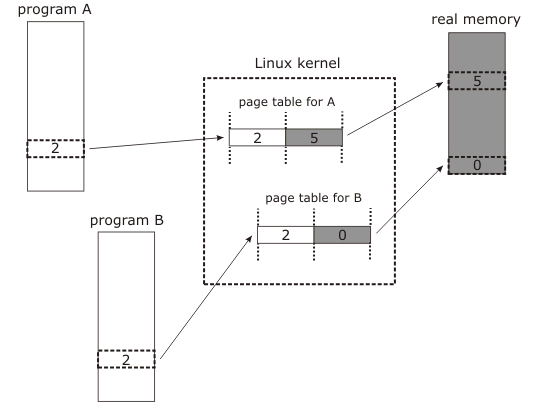
\includegraphics[width=\textwidth,keepaspectratio]{fig/vm}
	\caption{Překlad adres}
	\label{vm}
\end{figure}
\end{frame}

%%%
 \begin{frame}
\frametitle{Swapování stránek}
\begin{itemize}
\item Řeší záhadu proč může každý proces používat 4GB paměti i když je fyzicky nainstalováno méně RAM
\item Pokud je hlavní paměť RAM plná, jádro OS vybere nejméně potřebnou stránku a uloží ji na swap oddíl, typicky na sekundárním úložišti:
	\begin{itemize}
		\item v Linuxu obvykle samostatný diskový oddíl typu swap
		\item ve Windows stránkovací soubor viditelný přímo na disku
	\end{itemize}
\item Poté toto uvolněné místo ve fyzické paměti nahradí novou požadovanou stránkou
\item Při přístupu na stránku umístěnou ve swapu je stránka opět nahrána do hlavní paměti, kde opět vystřídá jinou, "nejméně" potřebnou, pokud není stále volné místo.
\item V designu paměťového podsystému je vždy velká snaha pomoci použití sofistikovaných algoritmů omezit použití swapu na minimum
\end{itemize}
\end{frame}

%%%
 \begin{frame}
\frametitle{Virtuální mapování uživatelských procesů}
\begin{itemize}
\item Každý spuštěný proces v OS obsahuje ve své virtuální paměti tyto namapované segmenty:
	\begin{description}
		\item[text] instrukce procesu
		\item[data] statické data a literály
		\item[heap] "halda", paměť určená k uživatelské alokaci, např. \texttt{malloc()/free()}
		\item[stack] zásobník používaný pro argumenty funkcí a lokální proměnné
	\end{description}
\item Pomocí utility \texttt{pmap} lze jednotlivé segmenty paměti jednoduše rozpoznat.
\end{itemize}
\end{frame}

%%%
 \begin{frame}[fragile]
\frametitle{Použití pmap}
\begin{verbatim}
[root@thinkpad-work imem_slides]# pmap 729
729:   /usr/sbin/irqbalance
0000000000400000     32K r-x--  /usr/sbin/irqbalance
0000000000607000      4K r----  /usr/sbin/irqbalance
0000000000608000      8K rw---  /usr/sbin/irqbalance
000000000250a000    132K rw---    [ anon ]
000000326d800000     40K r-x--  /usr/lib64/libnuma.so.1
000000326da0a000      4K rw---  /usr/lib64/libnuma.so.1
0000003904600000     16K r-x--  /usr/lib64/libcap-ng.so.0
0000003904604000   2044K -----  /usr/lib64/libcap-ng.so.0
...
00007fffb7c02000    132K rw---    [ stack ]
00007fffb7c67000      8K r-x--    [ anon ]
ffffffffff600000      4K r-x--    [ anon ]
 total            21076K
\end{verbatim}
\end{frame}

%%%
 \begin{frame}
\frametitle{Operace nad pamětí v jazyce C}
\begin{description}
\item[malloc()] alokace paměti na "haldě", přidání/rozšíření virtuálního mapování, vrací pointer
\item[free()] uvolnění alokované paměti, odstranění mapování
\item[mmap()] obecná funkce pro vytvoření mapování, lze použít pro anonymní paměť, pro soubory, i pro zařízení
\item[munmap()] zrušení mapování
\item[mlock()] označená paměť určená pointerem a délkou bude vždy umístěna v hlavní paměti, nebude nikdy odswapována
\item[munlock()] paměť jde opět odswapovat
\end{description}
\end{frame}

%%%
 \begin{frame}
\frametitle{Co se stane po zavolání malloc()?}
\begin{enumerate}
\item Jádro OS ověří, zda proces nepřekročil povolenou celkovou velikost a počet mapování
\item Vytvoří nebo rozšíří některé z existujících mapování stejného typu - tedy anonymní
\item Dokud do nově alokované paměti nebude přistupováno, fyzicky se nic alokovat nebude
\item Po zápisu do této paměti se přiřadí volný fyzický rámec k virtuální stránce a vytvoří se záznam v tabulce stránek
\item Pokud je první přístup čtení, odkazuje tabulka stránek k obecné vynulované stránce (zero-page)
\end{enumerate}
\end{frame}

%%%
%%%
\begin{frame}[fragile]
\frametitle{Ukázka}
\begin{verbatim}
int main(void)
{
	char *mem;

	mem = (char *) malloc(4096 * sizeof(char));
	if (!mem)
		return 1;

	bzero(mem, SIZE);
...
	free(mem);
\end{verbatim}
Kolik stránek bude programem na haldě fyzicky naalokováno po volání \texttt{bzero}?
Kolik stránek bude programem na haldě fyzicky naalokováno po zakomentování \texttt{bzero}?
\end{frame}

%%%
 \begin{frame}
\frametitle{Literatura}
\begin{itemize}
\item What Every Programmer Should Know About Memory, Ulrich Drepper, 2007 - ke stažení na \url{www.akkadia.org/drepper/cpumemory.pdf}
\item Computer Architecture, Fifth Edition: A Quantitative Approach,  Hennessy \& Patterson, 2011
\item \url{http://www.ualberta.ca/CNS/RESEARCH/LinuxClusters/mem.html}
\item \url{http://www.kernel.org/} (adresář \texttt{mm/})
\end{itemize}
\end{frame}


\end{document}
